% Poisoning the Deception Loop -- paper skeleton.
%
% Template: ACM sigconf (AISec uses ACM format), chosen provisionally per docs/PAPER_PLAN.md
% ("Confirm the venue, template and page limit before day 4"). To swap to USENIX later:
%   1. Replace the \documentclass line and the two acmart-specific commands below
%      (\acmConference..., \settopmatter...) with a usenix2019.sty preamble.
%   2. Everything from \input{sections/...} down is template-agnostic and needs no changes --
%      the section files contain only \section/\subsection structure, prose and floats.
% Build: .tools/tectonic.exe paper/main.tex   (or: python scripts/run.py figures && <same>)
\documentclass[sigconf,anonymous=false,review=false]{acmart}

\settopmatter{printacmref=false}
\renewcommand\footnotetextcopyrightpermission[1]{}
\pagestyle{plain}

% ---- venue / title / authors (placeholders; DECIDE at "Venue, template and page limit
% confirmed", docs/PAPER_PLAN.md "Open items") ----------------------------------------------
\acmConference[AISec '26]{ACM Workshop on Artificial Intelligence and Security}{TBD}{TBD}
\acmYear{2026}
\copyrightyear{2026}
\acmISBN{TBD}
\acmDOI{TBD}
\settopmatter{printccs=false}

\title{Poisoning the Deception Loop: Label Conflict in Honeypot-Fed Intrusion Detection}
% Working alternate title (docs/PAPER_PLAN.md): "When the Honeypot Writes the Labels:
% Poisoning Self-Training Intrusion Detectors"

\author{Author One}
\affiliation{%
  \institution{TBD}
  \city{TBD}
  \country{TBD}
}
\email{TBD}

\begin{abstract}
% docs/PAPER_PLAN.md "The claim, in one paragraph" -- draft here once prose starts.
% Do not draft prose yet (per instruction); this is a structural placeholder only.
TODO: abstract.
\end{abstract}

\begin{document}
\maketitle

\section{Introduction}
\label{sec:introduction}
% Source: docs/RELATED_WORK.md category A, DECISIONS.md s23, s26.1, s26.3, s26.5. Budget: 1 page.

A machine-learning intrusion detector needs labeled malicious traffic to train on, and labeled
malicious traffic is expensive: someone has to attack the network, or wait for someone else to,
and then confirm what happened. Honeypots offer an appealing shortcut. A decoy has no production
purpose, so nothing legitimate should ever reach it; whatever does is unsolicited by definition,
and can be auto-labeled malicious with no human in the loop. Feed that traffic into a detector's
training set and retrain periodically, and the detector adapts to new attack traffic without
anyone hand-labeling a single flow. This design is not hypothetical. Recent systems build
exactly this loop: \citet{matcheswala2024creating} pairs an adaptive honeypot with a network
traffic classifier trained on what the honeypot collects, and \citet{lanka2024intelligent}
applies machine-learning analysis to honeypot-collected data for threat detection. Neither
system asks what happens if the traffic reaching the decoy is not what the auto-labelling policy
assumes it is.

The assumption the whole design rests on is that the label is trustworthy \emph{because} the
source is a decoy. That assumption does not survive contact with an adversary who knows the
policy. The labelling rule — "everything the honeypot sees is malicious" — is public by
construction; there is no way to run the defense without publishing it, since the honeypot has
to be reachable to do its job. An attacker who knows the rule does not need to compromise
anything to write into the defender's training set: sending traffic to the decoy \emph{is}
writing to the training set, with a label the defender chooses to trust unconditionally. The
honeypot is not a passive sensor in this design; it is a write channel the defender opens on
purpose, and the poison budget available through it is not a fraction an attacker has to fight
for — it is the entire honeypot-derived share of the training set, by construction
(Section~\ref{sec:threat-model}).

This paper characterises that channel on a modern, flow-based network intrusion detection loop:
seed data plus honeypot traffic, retrained periodically, scored against held-out production
traffic. We confirm first that the loop does what it claims when the honeypot sees genuine
attacks — the honest case, S0, has to work before an attack on it means anything
(Section~\ref{sec:attack}). We then attack it with A1, benign mimicry: point the same traffic
generator that produces legitimate benign flows at the honeypot instead of production, and let
the auto-labeller do the rest. The result is one mechanism — a label that contradicts the
neighbourhood it sits in — that surfaces as false positives under a fixed detection threshold or
as lost detection under a recalibrated one, not two independent effects; recalibrating relocates
where the damage shows up, it does not remove it. On CICIDS2017 the attack requires
near-duplicate mimicry fidelity and needs no model access, no knowledge of the poison ratio, and
no cost to the attacker beyond producing traffic that already looks like traffic the network
generates for free. We hold every quantitative claim in this paper to a pre-registered,
multiple-comparison-corrected significance bar, and where a pattern in the data does not clear
that bar we report it as unconfirmed rather than round it up to a finding.

We then evaluate defenses. A generic label-consistency check — does this row's stamped label
agree with a model fit on the loop's own data — fails structurally against this attack, because
the poison is not inconsistent with anything the loop itself believes; it agrees with the
defender's own labelling policy, which is exactly what makes it hard to catch from inside the
loop. Cost-of-influence weighting, which we set out to propose as this paper's defense, does not
survive its own pre-registered evaluation: it fails a sensitivity criterion fixed in advance and
does not beat a matched no-skill baseline. What does work, and costs almost nothing to deploy,
is capping the honeypot's effective share of the training set — a one-line change that needs no
label information, no trusted reference data beyond the cap value itself, and no estimate of the
poison ratio, and that no alternative we test dominates. Along the way, measuring the attack on
CICIDS2017 exposes a property of the dataset itself: its benign traffic is narrow and repetitive
enough that an attacker gets most of the way to the damaging fidelity level for free, simply by
replaying the pool's own statistics with no perturbation at all — a fact about this benchmark's
degeneracy, not a general claim about production network traffic.

\subsection*{Contributions}
\begin{enumerate}
  \item A threat model for auto-labelled honeypot data as an attacker-controlled write channel
    into IDS training, characterised — mechanism, fidelity requirement, matched null controls —
    on a modern honeypot-fed retraining loop: the design that older signature-generator attacks
    targeted in a different form \cite{newsome2006paragraph,perdisci2006misleading}, and that
    current honeypot-plus-ML systems reintroduce without evaluating the threat
    (Section~\ref{sec:threat-model}).
  \item The attack characterised as one mechanism, surfaced as either false positives or lost
    detection depending on the threshold policy in force, not two independent channels; damage
    reported as a function of measured mimicry fidelity (twin fraction, not a jitter knob or a
    median distance too coarse to resolve the effect), held to a pre-registered,
    multiple-comparison-corrected significance bar throughout, including a dedicated,
    higher-powered follow-up that confirms one model's detection-loss damage extends well past
    copy-level fidelity, where a larger but lower-powered test could not resolve it
    (Section~\ref{sec:attack}).
  \item The policy-consistency blind spot: why a defense that checks a label's consistency
    against the loop's own data cannot catch poison that agrees with the loop's own labelling
    policy, and why a defense anchored to trusted data outside the loop can
    (Section~\ref{sec:defenses}).
  \item A defense comparison against a proper no-skill baseline: cost-of-influence weighting, our
    original proposal, is a measured negative result that does not beat it; a one-line cap on the
    honeypot's training-set share is undominated by every alternative tested and costs almost
    nothing to run (Section~\ref{sec:defenses}).
  \item A measurement of CICIDS2017's near-degeneracy under standard flow features, including
    that the attack's damage on this dataset traces to near-duplicate, not exact-duplicate,
    benign traffic, and what that implies for which claims this benchmark can and cannot support
    (Section~\ref{sec:degeneracy}).
\end{enumerate}

\begin{figure*}[t]
  \centering
  % F1: loop/threat diagram, drawn in TikZ (vector, no external tooling), not generated from
  % data. Colors match experiments/paper_figures.py's palette (loopblue = BLUE #2A78D6,
  % loopred = RED #E34948, loopmut = MUT #8A8A86, defined in main.tex) so F1 reads as the same
  % document as F2-F6. Source: CLAUDE.md architecture diagram + Section~\ref{sec:threat-model}.
  % Tried single-column (3.33in) first; two labeled inputs, a 4-stage pipeline, and two separate
  % evaluation callouts do not stay legible at that width, so this is figure* (full width).
  \begin{tikzpicture}[
      font=\sffamily\footnotesize,
      node distance=6mm and 7mm,
      box/.style={draw=loopblue, fill=loopbluebg, rounded corners=2pt, minimum height=8mm,
                  text width=20mm, align=center, thick, inner sep=2pt},
      hpbox/.style={box, draw=loopred},
      evalbox/.style={draw=loopmut, fill=white, dashed, rounded corners=2pt, minimum height=8mm,
                       text width=20mm, align=center, inner sep=2pt},
      arr/.style={-{Stealth[length=2mm]}, thick, draw=black!70},
    ]
    % --- inputs ---
    \node[box] (seed) {\texttt{seed\_train}\\[1pt]\lbl{trusted, defender-controlled}};
    \node[hpbox, below=of seed] (pool) {\texttt{honeypot\_pool}\\[1pt]\lbl{attacker sends traffic here}};

    % --- attacker-controlled pipeline ---
    \node[hpbox, right=of pool] (label) {auto-label\\[1pt]``malicious''};
    \node[box, right=of label] (defense) {defense hook\\[1pt]\lbl{optional, e.g. ShareCap}};

    % --- shared pipeline ---
    \node[box, right=16mm of $(label)!0.5!(defense)$, yshift=9mm] (accum) {accumulate};
    \node[box, right=of accum] (retrain) {retrain\\[1pt]\lbl{cold-start each round}};
    \node[box, right=of retrain] (detector) {detector};
    \node[box, right=of detector, text width=24mm] (score) {scores production traffic};

    % --- evaluation, off to the side, never touched by the loop ---
    \node[evalbox, below=10mm of detector] (evalset) {\texttt{trusted\_eval}\\[1pt]\lbl{held out, never written by the loop}};
    \node[evalbox, right=of evalset, text width=24mm] (thresh) {fixed vs.\ recalibrated threshold};

    % --- arrows ---
    \draw[arr] (seed.east) -| ($(seed.east)!0.5!(accum.west)$) |- (accum.west);
    \draw[arr] (pool) -- (label);
    \draw[arr] (label) -- (defense);
    \draw[arr] (defense.east) -| ($(defense.east)!0.5!(accum.west)$) |- (accum.west);
    \draw[arr] (accum) -- (retrain);
    \draw[arr] (retrain) -- (detector);
    \draw[arr] (detector) -- (score);
    \draw[arr] (evalset) -- (thresh);
    \draw[arr, loopmut] (evalset.north) -- (detector.south);
    \draw[arr, loopred, dashed] ($(pool.west)+(-9mm,3mm)$) node[font=\sffamily\scriptsize, loopred, anchor=east]{attacker} -- (pool.west);

    % --- attacker-controlled segment, marked ---
    \begin{pgfonlayer}{background}
      \node[draw=loopred, dashed, thick, rounded corners=4pt, fit=(pool)(label)(defense),
            inner sep=3mm, label={[loopred, font=\sffamily\scriptsize]above:attacker-controlled segment}] {};
    \end{pgfonlayer}
  \end{tikzpicture}
  \caption{The retraining loop. Everything the honeypot logs is auto-labeled malicious by a
  public policy and feeds the same \texttt{accumulate} step as trusted seed data (dashed red
  box: the attacker-controlled segment — the only traffic the attacker chooses is what the
  decoy sees, and that traffic becomes training data unconditionally). \texttt{trusted\_eval} is
  held out and never written by the loop; every result in this paper is scored against it under
  both a fixed and a recalibrated detection threshold.}
  \label{fig:loop-diagram}
\end{figure*}

\section{Background and Related Work}
\label{sec:background}
% Budget: 1 page. Four paragraphs:
%   1. Honeypot-ML integrations (cite closed-loop honeypot->IDS retraining papers).
%   2. Adaptive / LLM honeypots.
%   3. Poisoning of network classifiers.
%   4. Poisoning defenses.
% Plus two sentences on IDS dataset critiques (CICIDS2017 in particular -- ties to s5).
% End with the gap: nobody treats the honeypot's labels as untrusted.
% TODO: prose. TODO: references.bib entries.

\section{Threat Model}
\label{sec:threat-model}
% Budget: 0.75 page. Source: CLAUDE.md threat model, DECISIONS.md s4, s17.
% - Defender retrains on seed data plus honeypot traffic stamped malicious.
% - Attacker can send arbitrary traffic to the decoy, knows the labelling policy, cannot
%   touch production training data or the model.
% - Goals: raise false positives, or suppress detection.
% - Capability axis: mimicry fidelity, measured as realized NN distance to benign.
% TODO: prose.

\section{Methodology}
\label{sec:methodology}

\subsection{The loop}
% DECISIONS.md s7 (cold-start), s18 (retention/budget mode), s6 (one weight channel), s8 (seeds/determinism)
Each round: the adversary generates a batch of flows and a per-batch cost record (flows,
packets, bytes, flow-time); the auto-labeler stamps every row in the batch (Section~\ref{sec:threat-model});
a defense hook, when one is installed, sets a per-row \texttt{sample\_weight} and may quarantine
the whole batch; the batch is added to the accumulated training set; the model is
\textbf{retrained from scratch} on seed data plus every admitted batch to date; the fresh model
is scored on \texttt{trusted\_eval}. Retraining cold-start each round, rather than warm-starting
from the previous round's model, keeps rounds comparable and prevents poisoning dynamics from
being confounded with optimization path dependence.
% DECISIONS.md s18: retention=accumulate (default, worst case for the defender: honeypot
% influence never expires), budget_mode=fixed_ratio (the per-round batch size is set so the
% honeypot's share of the training set reaches a target ratio by the final round)
Two knobs govern how honeypot data accumulates. \emph{Retention} is \texttt{accumulate} by
default: every admitted batch is kept for the rest of the run, which is both the design the
honeypot-retraining literature proposes ("continuous adaptation") and the worst case for the
defender, since influence only grows. \emph{Budget mode} is \texttt{fixed\_ratio}: the
per-round batch size is set so the honeypot's share of the training set reaches a target ratio
by the final round, so every point on a damage curve has a known, comparable poison share.
% DECISIONS.md s6: single sample_weight channel; no class_weight="balanced", no scale_pos_weight,
% no oversampling/SMOTE -- A1 shifts the class balance by design, and automatic rebalancing would
% respond to that shift and confound the measured effect
No model in this codebase uses automatic class rebalancing (\texttt{class\_weight="balanced"},
XGBoost's \texttt{scale\_pos\_weight}, oversampling, SMOTE). A1 works by injecting
malicious-labeled volume, which shifts the class balance; an automatic rebalancer would respond
to that shift and the measured attack effect would be entangled with a rebalancing artifact.
\texttt{sample\_weight} is the only channel by which any row's influence on the fit is adjusted,
and every defense in Section~\ref{sec:defenses} rides on it.
% DECISIONS.md s8: seed_everything (Python, NumPy, PyTorch), deterministic kernels, float32
% features; the model seed varies by round (seed*1000+round) but is shared across arms at a
% given (seed, round), so paired same-seed deltas across arms isolate the treatment
Every fit seeds Python, NumPy and PyTorch and forces deterministic kernels. The model seed
varies by round but is shared across every arm at a given (seed, round), so a paired,
same-seed delta between an arm and the control isolates the treatment rather than retraining
noise.

\subsection{Datasets and partitions}
% DECISIONS.md s1: within_day_temporal splits within each (day, family) block, not each whole
% day, because a whole-day split places every attack family entirely inside one partition and
% destroys A4 as a variable. Fractions: benign 30/20/30/20, attack 40/-/40/20 (no prod_benign
% for attack). Four eval arms: seen_both / seed_only / honeypot_only / novel.
Data comes from CICIDS2017 (\texttt{MachineLearningCVE}) and a synthetic generator that ships
with the codebase, both partitioned identically into four disjoint sets: \texttt{seed\_train}
(the defender's trusted starting data), \texttt{prod\_benign} (unused here), \texttt{honeypot\_pool}
(what the adversary can draw from and what genuine decoy traffic would supply), and
\texttt{trusted\_eval} (held out, never written to by the loop). The split is within each
(day, family) block, not each whole day: benign rows go 30/20/30/20 to
seed\_train/prod\_benign/honeypot\_pool/trusted\_eval, attack rows 40/40/20 to
seed\_train/honeypot\_pool/trusted\_eval. This gives every attack family a presence in every
partition (\texttt{seen\_both}), which a whole-day split cannot, since CICIDS2017 runs each
family on its own day.
% PAPER_PLAN.md writing rule + DECISIONS.md s14 erratum: MachineLearningCVE has no Timestamp
% column; clean_flows synthesizes one at one row per second in file order. Every "temporal"
% split, guard-(b) buffer and burst boundary on CICIDS in this paper is therefore a file-order
% cut, not a wall-clock one.
\textbf{The CICIDS split is not temporal.} The \texttt{MachineLearningCVE} CSVs carry no
timestamp column; a timestamp is synthesized at one row per second in file order. Every cut,
buffer and burst boundary computed on CICIDS in this paper is therefore a file-order cut, not
a wall-clock one. Section~\ref{sec:degeneracy} shows this distinction does not matter to the
result: a uniformly shuffled re-split reproduces the same feature-space distances.
% DECISIONS.md s3: seed_only must never be merged with novel -- only seed_only is a controlled
% manipulation (A4), and collapsing it hides A4 entirely.
Four eval-family arms are tracked, never folded into an aggregate: \texttt{seen\_both} (in both
seed\_train and honeypot\_pool, the literature's regime), \texttt{seed\_only} (A4's controlled
arm), \texttt{honeypot\_only} (the loop's most interesting arm: a family the detector saw only
via the decoy), and \texttt{novel} (in neither).

% DECISIONS.md s24(b) + synthetic.py docstring: the generator emits raw-CICIDS-shaped data
% with well-separated class geometry (so a clean S0 loop can demonstrably improve) and injects
% the same corruption classes the real CSVs carry (NaN/Inf rates, negative durations, duplicate
% rows) so the cleaning pipeline is exercised end to end. It has no model of attacker effort or
% cost -- every synthetic flow's duration/packets/bytes come from the same class-conditional
% distribution regardless of scenario, which is why Section~\ref{sec:defenses}'s cost-based
% defense cannot separate benign from attack rows on this dataset.
The synthetic generator emits data in the same shape as the real CSVs, with well-separated
class geometry so a clean loop can demonstrably improve, and injects the same corruption
classes (non-finite rates, negative durations, duplicate rows) so the cleaning pipeline is
exercised the same way on both datasets. It has no model of attacker cost: a flow's duration,
packet count and byte count are drawn from the same class-conditional distribution regardless
of which scenario produced it.

\begin{table}[t]
  \centering
  \caption{Partition sizes (rows), near-duplicate grid 0.005. Attack rows have no
  \texttt{prod\_benign} share.}
  % Source: results/phase0/cicids/partition_summary.csv, results/phase0/partition_summary.csv
  \label{tab:partitions}
  \small
  \begin{tabular}{lrrrr}
    \toprule
    Partition & \multicolumn{2}{c}{CICIDS2017} & \multicolumn{2}{c}{Synthetic} \\
    & benign & attack & benign & attack \\
    \midrule
    seed\_train      & 344{,}823 & 78{,}877  & 20{,}383 & 8{,}241 \\
    prod\_benign     & 229{,}139 & --        & 13{,}098 & --      \\
    honeypot\_pool   & 344{,}221 & 130{,}166 & 19{,}951 & 7{,}993 \\
    trusted\_eval    & 229{,}695 & 52{,}054  & 13{,}262 & 4{,}535 \\
    \bottomrule
  \end{tabular}
\end{table}

\subsection{Leakage guards}
% DECISIONS.md s2: three guards on within_day_temporal -- (a) global near-duplicate removal
% (two half-offset grid snaps, grid 0.005 -- s11, s15), (b) a temporal guard band around
% internal cut times, (c) nearest-neighbour distance from every trusted_eval row to its
% nearest honeypot_pool row of the same class, reported as a percentile distribution for BOTH
% classes but gating leak_warning on the ATTACK class only.
Three guards run on every partition build. (a) Near-duplicate rows are removed globally, before
splitting, at grid resolution 0.005 (grid sweep and rationale in
Appendix~\ref{sec:appendix}). (b) Rows within a buffer of an internal cut are dropped
(burst-level splitting, a stronger version of this guard, is also in the appendix; it does not
change Section~\ref{sec:degeneracy}'s result). (c) For every \texttt{trusted\_eval} row, the
nearest-neighbour distance in normalized feature space to its nearest \texttt{honeypot\_pool}
row of the same class is computed and reported for both classes — this is the metric behind
every "realized distance" and "twin fraction" number in this paper.
% DECISIONS.md s2, s15: leak_warning gating rationale moved to Appendix for space; guard (c)'s
% definition above is kept in the main body since S5/S6 depend on readers knowing what it is.
Why the resulting \texttt{leak\_warning} is gated on the attack class alone, and what that does
and does not imply about the benign side, is in Appendix~\ref{sec:appendix}.

\subsection{Threshold policy}
% DECISIONS.md s5: calibrate to a target FPR (0.01) on a benign-stratified validation split
% carved from training, conservative under ties. Two modes, both reported: fixed (round-0
% threshold held) shows A1 damage as rising FPR; recalibrated (every round) shows it as
% collapsing TPR.
No model uses a 0.5 cutoff. Each model's threshold is calibrated to a target FPR (0.01) on a
validation split carved from its own training data. Two threshold modes are reported for every
run, because A1's damage surfaces in different places under each: \emph{fixed} calibrates once
at round 0 and holds that threshold, so damage appears as rising FPR on trusted benign;
\emph{recalibrated} recalibrates every round on trusted benign, so FPR stays capped by
construction and damage appears as collapsing TPR instead.
% DECISIONS.md s19.1: the round-0 validation split is full of near-copies of training rows on
% CICIDS (s16), so naive calibration is optimistic and the threshold too low. Fix: calibrate
% only on validation rows with no same-class training twin within tau=0.1 (per-feature RMS,
% normalized space). This discards 94% of benign validation rows and moves control fixed-FPR
% from 0.046 to 0.007 (RF).
On CICIDS2017 this calibration is not honest by default: the validation split is carved from
training data that, by Section~\ref{sec:degeneracy}'s measurement, is full of near-copies of
what it is meant to hold out, so a threshold calibrated against it is optimistic and lands too
low (control fixed-threshold FPR 0.046 against a 0.01 target). We calibrate instead only on
validation rows with no same-class training twin within a distance $\tau=0.1$ (the same
per-feature RMS metric as guard (c)). This discards 94\% of benign validation rows and moves
the control's fixed-threshold FPR to 0.007. Every CICIDS number in this paper after
Section~\ref{sec:degeneracy} uses this calibration.

\subsection{Arms}
% DECISIONS.md s23 table + s19.2: control (no ingestion, retrain on seed_train each round only,
% model seed varies by round so it measures real retrain noise); S0 (genuine attack rows,
% correctly labeled); A1 (benign rows, jittered, stamped malicious); plus three matched null
% controls that each remove one candidate mechanism: a1truth (the same rows as A1, true label:
% removes the label conflict), s0j (attack rows with A1's jitter, stamped malicious: same
% volume and prior shift, no label conflict), junk (marginal-shuffled bulk, stamped malicious:
% volume alone, no structure).
Every experiment compares an arm against a same-seed \emph{control} (no honeypot ingestion,
retrain on seed\_train alone each round; the model seed still varies by round, so the control
measures real retrain-to-retrain noise, not zero). \textbf{S0} (clean) feeds genuine attack
rows, correctly labeled. \textbf{A1} (benign mimicry) feeds benign rows, jittered by a
controlled amount, stamped malicious by the auto-labeler. Section~\ref{sec:attack} isolates
A1's mechanism with three matched null controls, each removing exactly one candidate cause:
\texttt{a1truth} (A1's own rows, correctly labeled — removes the label conflict),
\texttt{s0j} (attack rows carrying A1's jitter, stamped malicious — same volume and class-prior
shift, no label conflict), and \texttt{junk} (marginal-shuffled bulk, stamped malicious — volume
with no structure at all).

\subsection{Models, grids and metrics}
% DECISIONS.md s24 "Grid": RF and XGBoost hyperparameters (FAST_HYPERPARAMS in
% src/dloop/loop/rounds.py); 20 rounds, 5 seeds throughout.
Two models are trained per round: a random forest (25 trees, max depth 16) and XGBoost (60
trees), both at library defaults otherwise. Every result in this paper is 20 rounds, 5 seeds,
unless stated otherwise.
% src/dloop/loop/data.py LoopDataConfig defaults: seed_train_rows=30000,
% eval_benign_rows=40000, eval_attack_cap_per_family=4000 -- the fixed subsample the loop runs
% on each round (cheap enough to retrain from scratch every round, thousands of times over a
% sweep), drawn once per dataset and shared by every arm/seed/round so seed-to-seed variance
% reflects model and adversary randomness, not a changing evaluation set.
Each round retrains on a fixed subsample of the partitions in Table~\ref{tab:partitions}: up to
30{,}000 \texttt{seed\_train} rows, evaluated against up to 40{,}000 trusted benign rows and up
to 4{,}000 \texttt{trusted\_eval} rows per attack family, drawn once per dataset (not per seed)
so between-seed variance reflects model and adversary randomness rather than a moving
evaluation target.
% DECISIONS.md s4: A1 poison ratio grid is log-spaced, 0/0.005/0.01/0.02/0.05/0.1/0.2/0.5,
% because if A1 does real damage it shows at the low end and that is where resolution matters.
% Section 6's damage-vs-distance sweep uses ratios {0.05,0.1,0.2,0.5} and jitters
% {0,0.01,0.03,0.1,0.3,0.7,1.5}; s18: jitter is roughly log-spaced in REALIZED distance, and
% realized distance (not the jitter knob) is the reported x-axis.
The A1 poison-ratio grid is log-spaced (finer at the low end, where damage first appears if it
appears at all): $\{0, 0.005, 0.01, 0.02, 0.05, 0.1, 0.2, 0.5\}$ generally; the
damage-versus-distance sweep in Section~\ref{sec:attack} uses ratios
$\{0.05, 0.1, 0.2, 0.5\}$ and jitter $\{0, 0.01, 0.03, 0.1, 0.3, 0.7, 1.5\}$, roughly log-spaced
in \emph{realized} distance.
% DECISIONS.md s18 "Realized fidelity, not the knob": A1's x-axis is the median NN distance
% from the injected poison to the FULL trusted_eval benign set (guard-(c) metric, normalized
% space, per-feature RMS), computed per batch/round from the whole realized-distance
% distribution (p0-p100 recorded, median used for the x-axis); asserted disjoint from
% trusted_eval by row content.
The jitter knob is a generation parameter, not what is reported: every A1 plot's x-axis is the
\emph{realized} mimicry distance — the median nearest-neighbour distance (guard-(c) metric,
per-feature RMS, normalized space) from the injected poison rows to the full trusted benign
set, measured directly, not assumed from the jitter setting.
% DECISIONS.md s24 "Axes": R = 1 - mean(dFPR_defended)/mean(dFPR_undefended), A1 raw fidelity
% (jitter 0), ratio 0.5, fixed threshold. U = mean(gain_defended)/mean(gain_undefended), S0 on
% synthetic, honeypot_only TPR gain over control, ratios 0.05 and 0.2, fixed threshold.
Section~\ref{sec:defenses} reports two summary quantities against these arms. \emph{Recovery},
$R = 1 - \overline{\Delta\text{FPR}}_{\text{defended}} / \overline{\Delta\text{FPR}}_{\text{undefended}}$,
is measured on A1 at raw benign fidelity (jitter 0), poison ratio 0.5, fixed threshold — the
setting where undefended damage is largest. \emph{Retention},
$U = \overline{\text{gain}}_{\text{defended}} / \overline{\text{gain}}_{\text{undefended}}$, is
the honest loop's own \texttt{honeypot\_only} TPR gain over control on S0 (synthetic, ratios
0.05 and 0.2, fixed threshold), defended over undefended: how much of the honest loop's benefit
a defense leaves intact.
% DECISIONS.md s8: paired same-seed deltas at the final round; every table/figure delta in this
% paper is arm_metric[seed] - control_metric[seed], same seed, same round, then mean/sd over
% the 5 seeds and a paired t = mean / (sd / sqrt(5)).
Every reported delta is paired by seed: for each of the 5 seeds, an arm's final-round metric
minus the control's final-round metric at that same seed, then the mean, standard deviation and
paired $t = \bar{d} / (s_d/\sqrt{5})$ over the 5 differences.

\section{CICIDS2017 Is Near-Degenerate}
\label{sec:degeneracy}
% Budget: 0.75 page. Source: DECISIONS.md s10, s15, s16; results/phase0/cicids/nn_by_family.csv,
% grid_sweep.csv.
% - Every family with >500 eval rows, and benign, sits far below the leakage threshold at every
%   dedup grid and with burst splitting.
% - Consequence: no learning claim on CICIDS; S0 learning claim made on synthetic instead.
% - The 94% of benign validation rows discarded for an honest threshold (s23).
% TODO: prose.

\begin{figure}[t]
  \centering
  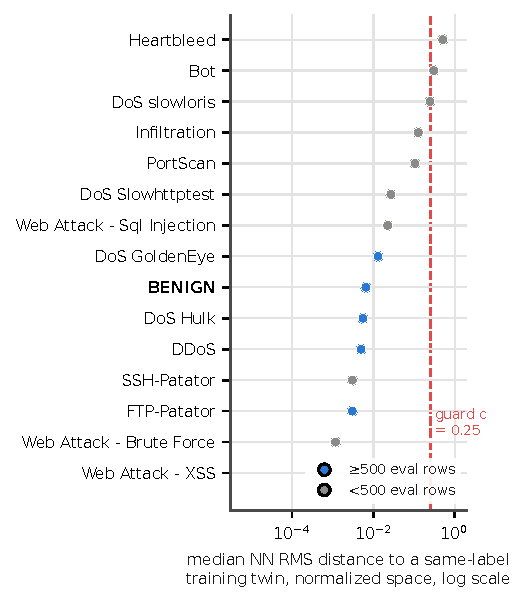
\includegraphics[width=\linewidth]{figures/F2_nn_by_family.pdf}
  % Source: results/phase0/cicids/nn_by_family.csv + leakage_report.json (benign row).
  % Regenerated by: python scripts/run.py figures --only F2  (experiments/paper_figures.py:fig_f2)
  \caption{TODO caption. Per-family median nearest-neighbour RMS distance to a same-label
  training twin (log scale); families with fewer than 500 trusted\_eval rows greyed out as
  not reportable. Dashed line: the guard-(c) leakage threshold, 0.25.}
  \label{fig:f2-nn-by-family}
\end{figure}

\section{The Attack}
\label{sec:attack}
% Budget: 1.5 pages. Source: DECISIONS.md s17, s19, s22, s23; results/phase0/loop/,
% results/phase0/mechanism/.
% - S0 works: honeypot_only 0.4 -> 0.99 on synthetic.
% - A1 damage vs mimicry distance: cliff at ~0.011-0.014 for the FPR channel.
% - Two channels (s23 table): FPR needs copy fidelity and >=10-20% poison; RF's TPR channel
%   works at every distance tested; XGBoost has no TPR channel.
% - Mechanism isolation: a1truth, s0j, junk all null.
% - Recalibrating trades FPR damage for TPR loss.
% - XGBoost FPR channel seed-dependent, reported per seed (DECISIONS.md s25.6).
% TODO: prose.

\begin{figure}[t]
  \centering
  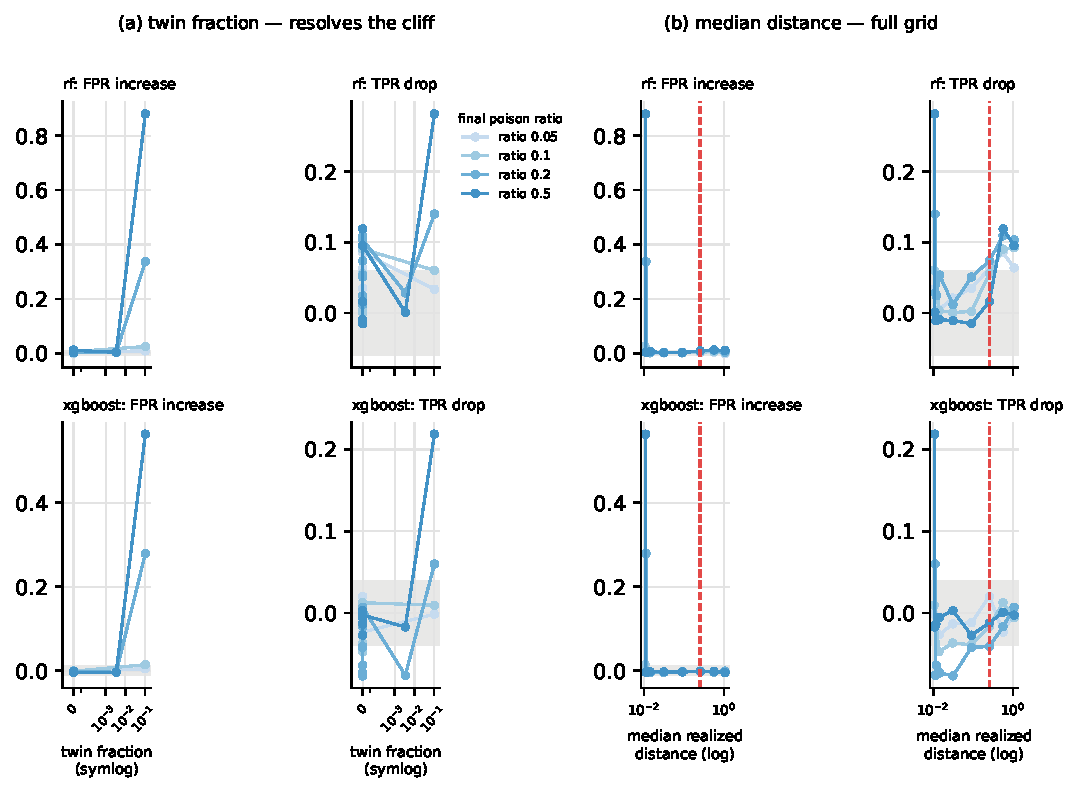
\includegraphics[width=\linewidth]{figures/F3_damage_vs_fidelity.pdf}
  % Source: results/phase0/loop/cicids/a1_damage_vs_fidelity.csv, s0_reference_damage.csv.
  % Regenerated by: python scripts/run.py figures --only F3  (experiments/paper_figures.py:fig_f3)
  \caption{TODO caption. A1 damage vs.\ realized mimicry distance to trusted benign (log scale),
  RF and XGBoost, fixed-threshold FPR and recalibrated-threshold TPR. Grey band: $\pm2\sigma$ of
  the control's own round-to-round variance. Dotted: S0 (genuine attacks) at the same ratio.}
  \label{fig:f3-damage-vs-fidelity}
\end{figure}

\begin{figure}[t]
  \centering
  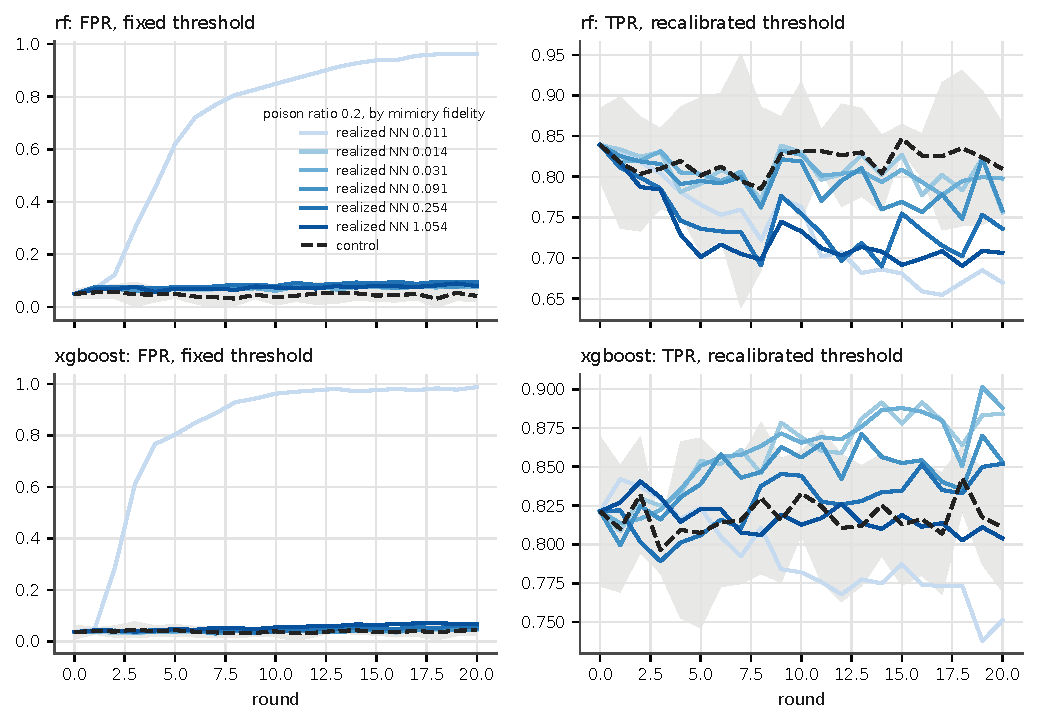
\includegraphics[width=\linewidth]{figures/F4_a1_trajectory.pdf}
  % Source: results/phase0/loop/cicids/jobs/*.csv (per-seed, per-round; undefended, tau=0).
  % Regenerated by: python scripts/run.py figures --only F4  (experiments/paper_figures.py:fig_f4)
  \caption{TODO caption. A1 on CICIDS2017 at poison ratio 0.2: per-round FPR (fixed threshold)
  and TPR (recalibrated threshold), by realized mimicry fidelity. Dashed: control mean
  $\pm2$\,sd across seeds.}
  \label{fig:f4-trajectory}
\end{figure}

\begin{figure}[t]
  \centering
  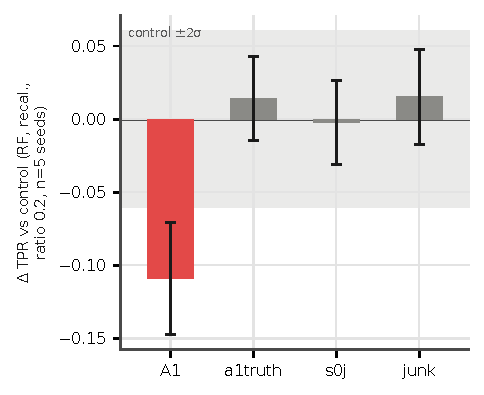
\includegraphics[width=\linewidth]{figures/F5_mechanism_isolation.pdf}
  % Source: results/phase0/export/summary.csv (rows: scenario in {a1,a1truth,s0j,junk},
  % model=rf, threshold_mode=recalibrated, target_poison_ratio=0.2, run_dir=cicids_recal).
  % Regenerated by: python scripts/run.py figures --only F5  (experiments/paper_figures.py:fig_f5)
  \caption{TODO caption. Mechanism isolation: $\Delta$TPR vs.\ control (RF, recalibrated
  threshold, ratio 0.2, $n=5$ seeds) for A1 and three null controls that each remove one
  candidate mechanism. Error bars: sd over seeds. Band: control's own $\pm2\sigma$.}
  \label{fig:f5-mechanism}
\end{figure}

\begin{table}[t]
  \centering
  \caption{TODO: the two channels. Source: DECISIONS.md s23 table.}
  \label{tab:two-channels}
  \begin{tabular}{lll}
    \toprule
    Channel & Model & Behavior \\
    \midrule
    FPR (false alarms) & RF, XGBoost & TODO \\
    TPR (detection loss) & RF only & TODO \\
    \bottomrule
  \end{tabular}
\end{table}

\section{Defenses}
\label{sec:defenses}
% Budget: 1.25 pages. Source: DECISIONS.md s20, s21.5, s23, s24.1, s25.3, s25.5.
% - Policy-consistency blind spot: loss filtering recovers ~0% (s23).
% - D1 as pre-registered; missed its own sensitivity criterion (s20, s21.5).
% - Frontier vs kNN and no-skill baselines; uniform fails at ratio 0.9 (s24.1).
% - ShareCap: undominated in all 87 comparisons; cap curve (s25.3, s25.5).
% - Overhead: D1 ~781x cheaper than kNN; ShareCap near zero.
% - Counter-moves: padding (s21.6), volume (s21.4).
% Writing rule (docs/PAPER_PLAN.md): never say D1 is effective, or that ShareCap "beats"
% others (it is undominated, not shown superior in every comparison).
% TODO: prose.

\begin{figure}[t]
  \centering
  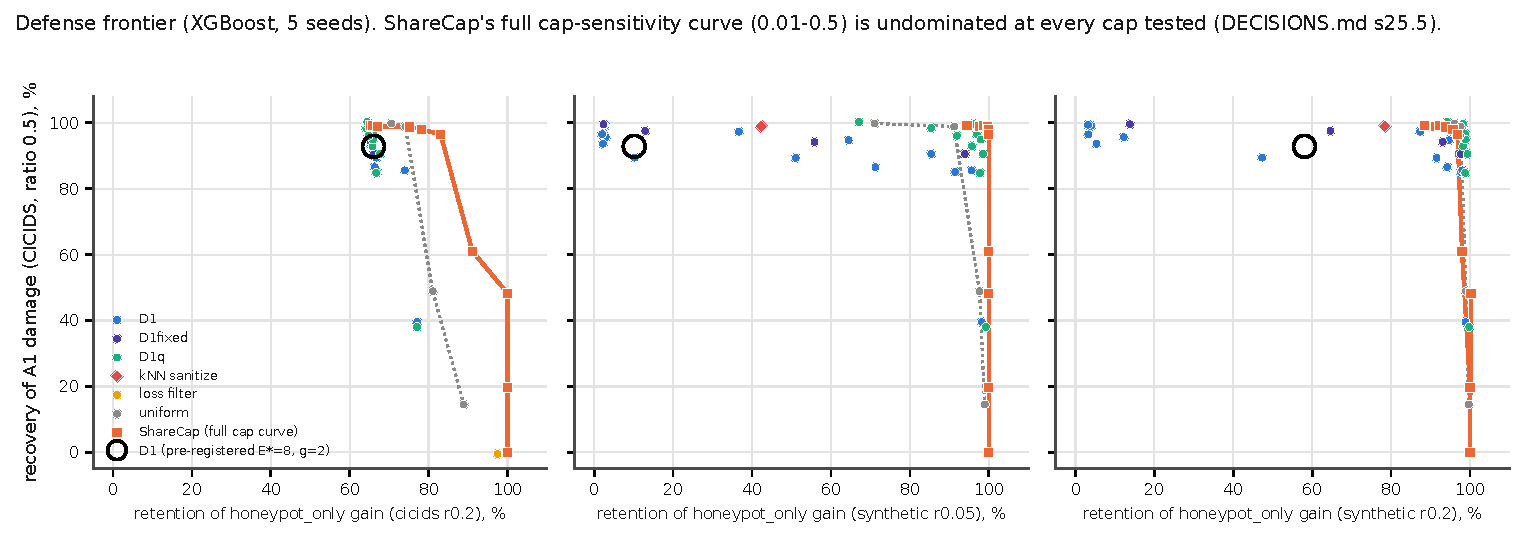
\includegraphics[width=\linewidth]{figures/F6_frontier.pdf}
  % Source: results/phase0/frontier/frontier_points.csv (D1/D1q/D1fixed/kNN/loss/uniform) +
  % results/phase0/loop/{cicids_recal,synthetic}/jobs/*sharecap_c*.csv (full ShareCap cap
  % curve, computed fresh in experiments/paper_figures.py:_sharecap_curve -- DECISIONS.md s25.5).
  % Regenerated by: python scripts/run.py figures --only F6
  \caption{TODO caption. Recovery of A1 damage (CICIDS, ratio 0.5) vs.\ retention of the
  honest loop's S0 gain, three retention axes. Points: D1 variants, kNN sanitize, loss
  filter, fixed-weight uniform down-weighting (dotted line: the no-skill baseline at each
  weight). Orange line: ShareCap's full cap-sensitivity curve, $c\in\{0.01,\ldots,0.5\}$.
  Circled: the pre-registered D1 configuration ($E^*=8,\gamma=2$).}
  \label{fig:f6-frontier}
\end{figure}

\begin{table}[t]
  \centering
  \caption{TODO: loss-filter recovery by ratio. Source: DECISIONS.md s23.}
  \label{tab:loss-filter}
  \begin{tabular}{lrr}
    \toprule
    Poison ratio & Recovery & Notes \\
    \midrule
    TODO & TODO & TODO \\
    \bottomrule
  \end{tabular}
\end{table}

\begin{table*}[t]
  \centering
  \caption{TODO: defense comparison. Source: DECISIONS.md s24.1, s25.3.}
  \label{tab:defense-comparison}
  \begin{tabular}{lrrrrr}
    \toprule
    Defense & Recovery r0.5 & Recovery r0.9 & Retention CICIDS & Retention synthetic & Overhead / round \\
    \midrule
    TODO & TODO & TODO & TODO & TODO & TODO \\
    \bottomrule
  \end{tabular}
\end{table*}

\section{Discussion and Limitations}
\label{sec:discussion}
% Budget: 0.5 page. Source: DECISIONS.md s16, s25.5, s25.6, s26.3, s26.5, s14 erratum.

\textbf{When this matters.} The attack needs benign traffic the adversary can reproduce with
near-duplicate fidelity, and CICIDS2017 makes that cheap because its own benign class is narrow
and repetitive (Section~\ref{sec:degeneracy}) — replaying the pool's own statistics with no
perturbation already lands one row in ten within twin-fraction range
(Section~\ref{sec:attack}). Production networks with genuinely diverse, high-entropy benign
traffic would raise the fidelity bar the attacker has to clear; networks that do not — IoT
fleets, ICS traffic, automated service-to-service calls, anything whose "normal" is a small set
of repeated request shapes — are closer to CICIDS2017's regime than to a diverse enterprise
network, and are where this channel should be expected to be cheapest to exploit. We do not
measure this on production traffic; it is a prediction from the mechanism, not a finding.

\textbf{Practical advice.} Cap the honeypot's effective share of the training set; it is the one
defense here that costs nothing to deploy, needs no label information or trusted reference data
beyond the cap value, and is undominated by every alternative we test
(Section~\ref{sec:defenses}). Do not trust a label-consistency check that learns from the loop's
own data to catch this poison — it cannot, because the poison is consistent with the loop's own
labelling policy by construction; a check anchored to data outside the loop can.

\textbf{Limitations.} This is an offline simulation of the loop, not a deployed system: the
adversary's batches are drawn from a fixed pool rather than generated against a live honeypot,
and there is no network-level cost to reaching the decoy in the first place. We measure flow
features only, not payload content, so any attack or defense that depends on packet contents is
out of scope. CICIDS2017 answers the degeneracy measurement and the fidelity-versus-damage curve
but carries no learning claim (Section~\ref{sec:degeneracy}); the synthetic dataset answers the
honest-loop learning claim but has no attacker-cost profile of its own. Five seeds is enough to
establish some effects and not others: XGBoost's fixed-threshold FPR trajectory splits into two
distinct per-seed groups rather than clustering around a mean (Section~\ref{sec:attack}), and
RF's damage at large mimicry distance needed a dedicated 15-seed follow-up to confirm — the
original 5-seed, 36-cell grid family lacked the power to resolve it, even though the effect was
real (Section~\ref{sec:attack}). We only had the budget to run that follow-up for RF; the same
question is open for XGBoost. Further limitations — the partition's file-order versus verified
timestamp, and ShareCap's cap range and adaptive-attacker coverage — are in
Appendix~\ref{sec:appendix}.

\section{Conclusion}
\label{sec:conclusion}
% Budget: 0.25 page.

Auto-labeling a honeypot's traffic and retraining a detector on it treats the label as free
because the source is a decoy. It is not free: the labelling policy is public, the attacker
chooses exactly what the decoy sees, and the honeypot becomes a write channel into the
defender's training set that the defender opened on purpose. We showed this channel is
exploitable on a modern, flow-based retraining loop with a single mechanism — a label that
contradicts its neighbourhood — that a fixed detection threshold reads as false positives and a
recalibrated one reads as lost detection, not two separate effects. The attack needs near-copy
mimicry fidelity and nothing else: no model access, no knowledge of the poison ratio, no cost
beyond producing traffic that already resembles what the network generates. A generic
label-consistency defense cannot see this poison because it agrees with the defender's own
policy; a one-line cap on the honeypot's share of the training set can, and beats every
alternative we compared it against without needing any of the information those alternatives
require. The honest version of this loop works — that was never in question — but the design
that makes it convenient, a public rule that trusts a decoy's traffic unconditionally, is the
same design that makes it attackable, and the fix costs almost nothing to add.


\bibliographystyle{ACM-Reference-Format}
\bibliography{references}

\appendix
\section{Appendix}
\label{sec:appendix}
% Source: DECISIONS.md s1 (day-split robustness), s14 (burst splitting), s11 (guard (a) grid
% sweep), s20 + s24 (D1 definition and full grid), s25.6 (XGBoost per-seed trajectories),
% s21.6 (padding), s25.5 (full cap curve -- already in Figure~\ref{fig:f6-frontier}, main body).
% TODO: prose, and decide which tables/figures move here vs. stay in the main body once the
% page budget is known (docs/PAPER_PLAN.md "Confirm the venue, template and page limit").

\subsection{Twin fraction: sensitivity to the chosen delta}
% Source: results/phase0/cicids/twin_fraction_by_jitter.csv (delta in {0.001, 0.0015, 0.003}).
% delta=0.0015 (Figure 3's value) was chosen from the s26.2 p5 gap; this checks whether the
% picture depends on that specific choice. It does, in one respect worth stating plainly: 0.003
% does not track the FPR collapse (s26.2: already at the noise floor by jitter 0.002) as tightly
% as the two finer deltas do.
Figure~\ref{fig:f3-damage-vs-fidelity}(a) uses $\delta=0.0015$, chosen from where the
realized-distance distribution's 5th percentile jumps between jitter 0 and jitter 0.002
(Section~\ref{sec:threat-model}). Table~\ref{tab:twin-delta-sensitivity} recomputes twin
fraction at $\delta\in\{0.001, 0.003\}$, bracketing that choice by roughly 2x in each direction.
The qualitative story — a cliff within one to two jitter steps of raw fidelity, not a gradient —
holds at all three, but the exact location is not delta-invariant: $\delta=0.001$ and
$\delta=0.0015$ both collapse to near-zero by jitter 0.002, matching where the FPR damage itself
disappears (s26.2); $\delta=0.003$ is coarse enough that it still reads 0.173 at jitter 0.002 —
comparable to $\delta=0.0015$'s own raw-jitter value — and does not fall to near-zero until
jitter 0.005, one step later than the damage does. A delta chosen too loosely lags the effect it
is meant to track; the finer two values, including the one used in Figure~\ref{fig:f3-damage-vs-fidelity},
do not.

\begin{table}[t]
  \centering
  \caption{Twin fraction by jitter, at three values of $\delta$.}
  \label{tab:twin-delta-sensitivity}
  \small
  \begin{tabular}{lrrr}
    \toprule
    Jitter & $\delta=0.001$ & $\delta=0.0015$ & $\delta=0.003$ \\
    \midrule
    0.000 & 0.057 & 0.105 & 0.212 \\
    0.002 & 0.00002 & 0.003 & 0.173 \\
    0.005 & 0.000 & 0.000 & 0.001 \\
    $\ge$0.01 & 0.000 & 0.000 & 0.000 \\
    \bottomrule
  \end{tabular}
\end{table}

\subsection{Guard (a): near-duplicate grid sweep, and why \texorpdfstring{\texttt{leak\_warning}}{leak\_warning} is attack-only}
% Source: DECISIONS.md s11 (grid sweep), s2/s15 (leak_warning gating rationale, moved here from
% Section 4 for space).
The near-duplicate guard (Section~\ref{sec:methodology}) removes a large fraction of the benign
class on CICIDS2017 at any reasonable grid resolution, so that resolution cannot be picked by
feel. Sweeping \texttt{near\_dup\_grid} $\in \{\text{off}, 0.005, 0.01, 0.02, 0.05\}$: with the
guard off, partition construction fails outright (CICIDS2017 has roughly 12.3k flows that are
row-content-identical, to six decimal places, across \texttt{seed\_train} and
\texttt{trusted\_eval}). From 0.005 to 0.05, benign rows removed range over $2\times$ and
\texttt{seed\_train} shrinks from 456k to 267k rows, but RF AUROC stays in 0.98--0.996 and TPR in
0.95--0.97 throughout; \texttt{leak\_warning} is set at every grid tested. The result does not
depend on which grid in this range is used, and the guard is necessary regardless of grid: this
paper uses 0.005 throughout.

\texttt{leak\_warning} itself is gated on the attack class alone, not benign. Guard (c)'s purpose
in setting that flag is to catch \texttt{S0} passing its checkpoint by memorization of a specific
held-out row rather than by learning a boundary; two different benign flows, unrelated to any
attack, can legitimately carry identical flow statistics (the same web request shape occurring
twice), so a near-zero benign nearest-neighbour distance is not by itself evidence of a leak the
way the same distance on the attack class would be. This does not mean the benign side is
ignored: guard (c) measures it on the same scale and reports it unconditionally, and
Section~\ref{sec:degeneracy} is built entirely on that benign-side measurement, because it bears
directly on A1 (whose poison and whose measured damage are both benign-side) and on the
threshold-calibration fix (Section~\ref{sec:methodology}).

\subsection{Burst splitting}
% Source: DECISIONS.md s14. Erratum embedded in s14 itself: CICIDS2017's MachineLearningCVE CSVs
% carry no Timestamp column, so every "gap"/"burst" here is a file-order run length, not a
% wall-clock inter-arrival time (same caveat as Section 4's "the CICIDS split is not temporal").
Section~\ref{sec:methodology}'s guard (b) is a row-level cut, which could in principle slice
through the middle of a contiguous burst of highly similar flows (a flood tool's output, most
obviously). Burst-level splitting tests this directly: segment each (day, family) stream into
contiguous episodes by inter-flow gap ($>2$s, chosen from the measured gap distribution) and
assign each burst whole to one partition, never dividing one across a boundary
(\texttt{tests/test\_partition.py} asserts this invariant on the reconstructed union of all four
partitions). Two family groups emerge: session-like families (Bot, SSH-/FTP-Patator, DoS
GoldenEye, Web Attack variants) have a median inter-flow gap of 4--38s and thousands of bursts
per day, where a row-level cut genuinely could split one; continuous floods (DoS Hulk, DDoS, DoS
Slowhttptest, PortScan) have a median gap under 1s and essentially do not pause — DDoS is
$\sim$128k rows in 22 bursts for the entire day.

With burst splitting on, the guard-(a) grid sweep repeats at the same order of magnitude as the
row-level cut ($\text{nn\_attack\_p5}$ 0.0010--0.0058 across grid 0.005--0.05, versus 0.0010--0.0067
row-level, Section~\ref{sec:degeneracy}); \texttt{leak\_warning} is set at every grid, unchanged.
The per-family nearest-neighbour breakdown explains why burst-awareness does not help: DoS
Hulk's nearest \texttt{honeypot\_pool} neighbour to a \texttt{trusted\_eval} row has RMS distance
0.0003, DDoS 0.00017, DoS GoldenEye 0.00017 — a different burst, sometimes a different half of
the day, and the feature vector is still within noise of zero distance. The degeneracy
(Section~\ref{sec:degeneracy}) is a property of the feature representation these families
produce, not an artifact of where or how the cut is drawn.

\subsection{D1: full definition and grid}
% TODO. Source: DECISIONS.md s20, s24.

\subsection{XGBoost per-seed trajectories}
% Source: DECISIONS.md s25.6. Full 8-round, both-model per-seed table; Section 6 summarizes
% this and refers here rather than reproducing all 10 rows in the main body.
Section~\ref{sec:attack} reports XGBoost's fixed-threshold FPR response to A1 as seed-dependent
rather than characterisable from a mean over 5 seeds; Table~\ref{tab:xgb-seeds-full} is the full
per-seed trajectory this is based on (ratio 0.5, raw fidelity, rounds 2 through 20). XGBoost is
bimodal: seeds 2 and 4 reach 70--84\% FPR by round 8--10; seeds 1 and 5 stay below 2\% through
round 10, and only seed 5 climbs at all by round 20 (to 12\%); seed 3 sits in between, jumping
late (round 6--8). RF climbs on all 5 seeds, with none staying flat. A mean-over-seeds summary
hides this: XGBoost's round-10 mean is dragged up by two seeds while three show no effect at
all, which is a bimodal outcome, not a noisy estimate of one common trajectory. Every mean
XGBoost number elsewhere in this paper should be read with that in mind.

\begin{table}[t]
  \centering
  \caption{Fixed-threshold FPR by seed and round, ratio 0.5, raw fidelity, both models.}
  % Source: DECISIONS.md s25.6 (results/phase0/loop/cicids_recal/jobs/a1_{model}_s*_j0.0_r0.5_vt0.1.csv).
  \label{tab:xgb-seeds-full}
  \small
  \begin{tabular}{llrrrrrrrr}
    \toprule
    Model & Seed & r2 & r4 & r6 & r8 & r10 & r12 & r15 & r20 \\
    \midrule
    XGBoost & 1 & 0.005 & 0.005 & 0.004 & 0.006 & 0.006 & 0.006 & 0.007 & 0.019 \\
    XGBoost & 2 & 0.016 & 0.503 & 0.737 & 0.782 & 0.823 & 0.878 & 0.924 & 0.955 \\
    XGBoost & 3 & 0.006 & 0.007 & 0.053 & 0.538 & 0.693 & 0.714 & 0.734 & 0.800 \\
    XGBoost & 4 & 0.046 & 0.707 & 0.776 & 0.839 & 0.908 & 0.949 & 0.948 & 0.958 \\
    XGBoost & 5 & 0.005 & 0.004 & 0.004 & 0.006 & 0.007 & 0.008 & 0.010 & 0.117 \\
    RF & 1 & 0.048 & 0.232 & 0.618 & 0.721 & 0.767 & 0.804 & 0.858 & 0.911 \\
    RF & 2 & 0.032 & 0.153 & 0.503 & 0.700 & 0.735 & 0.776 & 0.840 & 0.894 \\
    RF & 3 & 0.021 & 0.088 & 0.362 & 0.612 & 0.706 & 0.743 & 0.776 & 0.853 \\
    RF & 4 & 0.015 & 0.095 & 0.383 & 0.615 & 0.728 & 0.740 & 0.788 & 0.869 \\
    RF & 5 & 0.042 & 0.284 & 0.647 & 0.729 & 0.779 & 0.836 & 0.880 & 0.917 \\
    \bottomrule
  \end{tabular}
\end{table}

\subsection{Cost padding}
% TODO. Source: DECISIONS.md s21.6.

\subsection{Additional limitations}
% Source: DECISIONS.md s14 erratum (file-order split), s25.5 (cap is model/dataset-specific),
% s25.7 (session-level D1/adaptive-attacker parked, not run). Moved from Section 8 for space;
% these are real limitations, not lower-priority ones -- kept complete here rather than cut.
Beyond the four limitations in Section~\ref{sec:discussion}:

\begin{itemize}
  \item \textbf{The partition is by file order, not a verified capture timestamp.}
    CICIDS2017's public \texttt{MachineLearningCVE} release carries no timestamp column
    (Section~\ref{sec:methodology}), so "day split" in this paper means the dataset's own file
    boundaries, not confirmed calendar time. A burst-aware split gives comparable results
    (Appendix~\ref{sec:appendix}, "Burst splitting"), but that is evidence the result survives a
    different file-order cut, not independent evidence of separation on real wall-clock time.
  \item \textbf{ShareCap's safe cap range is not a universal constant.} It is measured for one
    model and one dataset at a time (Section~\ref{sec:defenses}); a different model or dataset
    may have a different safe range, and we do not have a way to predict it without measuring it.
  \item \textbf{No adaptive attacker against ShareCap beyond filling the cap.} We do not test an
    attacker who observes or infers the cap and tunes its poison ratio specifically around it,
    e.g. staying just under the cap indefinitely rather than pushing past it. Session-level
    cost-of-influence weighting (a defense that might address a session-aware version of this)
    was considered and parked, not run: the dataset that would carry the source IPs and
    timestamps it needs is form-gated and was unavailable to us.
\end{itemize}


\end{document}
